\documentclass{article}
\usepackage[T1]{fontenc}
\usepackage{lmodern}
\usepackage{graphicx}
\usepackage{amsmath,amssymb}
\usepackage[a4paper,margin=2cm]{geometry}
\usepackage[absolute,overlay]{textpos}
\setlength{\TPHorizModule}{1mm}
\setlength{\TPVertModule}{1mm}
\usepackage[indonesian]{babel}
\usepackage{hyperref}
\setlength{\emergencystretch}{2em}
% unit: Halaman 27

\begin{document}

% === Halaman 27 (llm) ===

\vspace{135.73mm}

(a) Skema enkripsi mode CBC

\begin{itemize}
    \item[Encryption:]
    \[ C_0 = \text{IV} \]
    \[ C_i = E_K (P_i \oplus C_{i-1}) \]
\end{itemize}

\vspace{30mm}

(b) Skema dekripsi mode CBC

\begin{itemize}
    \item[Decryption:]
    \[ C_0 = \text{IV} \]
    \[ P_i = D_K (C_i) \oplus C_{i-1} \]
\end{itemize}

% deskripsi: Diagram alur proses enkripsi Cipher Block Chaining (CBC) yang menunjukkan penggunaan Initialization Vector (IV), operasi XOR antara plaintext dan ciphertext sebelumnya, serta blok enkripsi E dengan kunci K.
% bbox normalisasi: [0.3020, 0.0250, 0.9450, 0.4820]
\begin{textblock*}{135.03mm}(63.42mm,7.43mm)
\noindent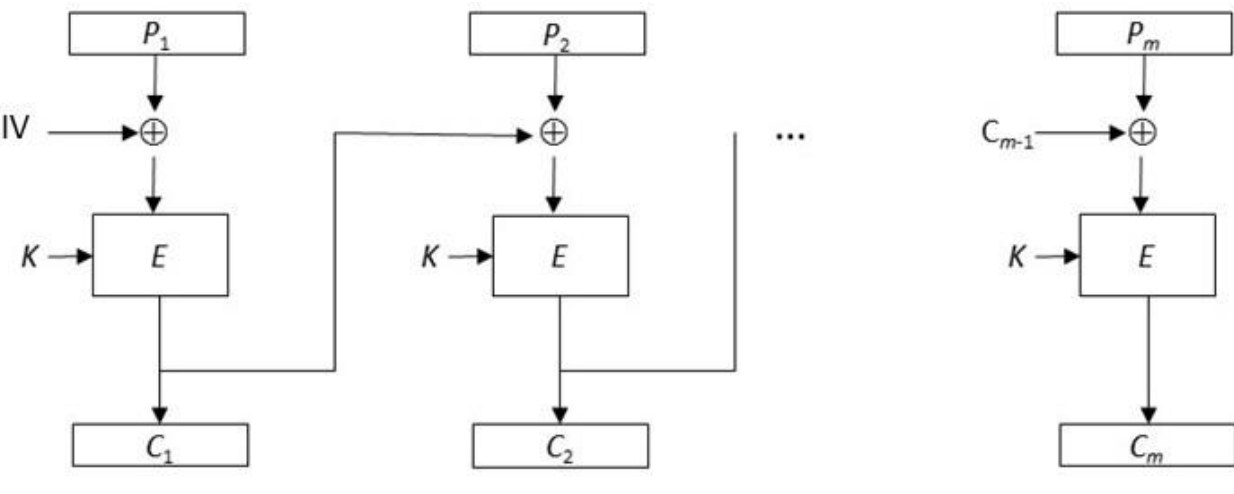
\includegraphics[width=135.03mm,height=135.73mm]{../../images/llm/page_027_img_01.png}%
\end{textblock*}

% deskripsi: Diagram alur proses dekripsi Cipher Block Chaining (CBC) yang menunjukkan penggunaan blok dekripsi D dengan kunci K, dan operasi XOR antara hasil dekripsi dengan ciphertext sebelumnya untuk mendapatkan plaintext.
% bbox normalisasi: [0.3020, 0.5350, 0.9450, 0.9700]
\begin{textblock*}{135.03mm}(63.42mm,158.90mm)
\noindent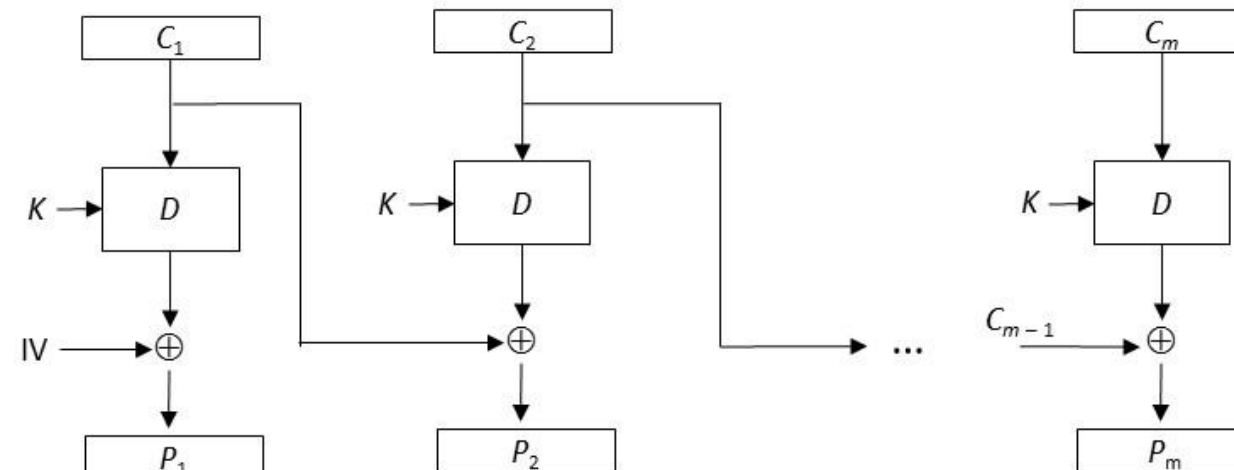
\includegraphics[width=135.03mm,height=129.19mm]{../../images/llm/page_027_img_02.png}%
\end{textblock*}

\end{document}
